\documentclass{article}
\usepackage[utf8]{inputenc}
\usepackage[T1]{fontenc}
\usepackage[english]{babel}
\usepackage{lmodern}
\usepackage{microtype}
\usepackage{graphicx}
\usepackage{float}
\usepackage{subcaption}
\usepackage{hyphenat}
\usepackage{natbib}
\usepackage{url}
\usepackage{amsmath}
\usepackage{booktabs}
\usepackage{tikz}
\usetikzlibrary{shapes.geometric, arrows.meta, positioning}
\captionsetup[subfigure]{skip=2pt, justification=centering}
\usepackage{xcolor}
\definecolor{blue!50}{RGB}{50,100,200}
\definecolor{green!50}{RGB}{34,140,34}
\definecolor{orange!50}{RGB}{200,100,50}
\setlength{\parindent}{0pt}
\setlength{\parskip}{6pt plus 2pt minus 1pt}

\begin{document}

\title{AI-based IGRT with 2D Image-Guided Dose Tracking of Daily Cone-Beam CTs for Evaluating Rectum and Bladder Filling in Definitive Radiotherapy for Prostate Carcinoma}

\author{%
\begin{minipage}{\textwidth}
\centering
\small
Peter Rhone, Dipl.-Phys.\textsuperscript{1}, 
Saskia Spautz, MSc\textsuperscript{2,3,*},\\ 
Annika Schlamann, MD\textsuperscript{2,3}, 
Thomas Kuhnt, MD, Prof.\textsuperscript{2,3},\\ 
Franziska Nägler, MD\textsuperscript{2,3,**} \\[1ex]
\footnotesize\textsuperscript{1}Clinic for Radiation Therapy and Radiooncology, Heinrich-Braun-Clinic Zwickau, \\ 
\footnotesize\textsuperscript{2}Clinic and Polyclinic for Radiation Therapy, University Hospital Leipzig \\ 
\footnotesize\textsuperscript{3}Central German Cancer Center (CCCG), Partner Site Leipzig \\ 
\footnotesize\textsuperscript{*}shared first authorship
\footnotesize\textsuperscript{**}senior author
\end{minipage}%
}
\maketitle 

\vspace{0.5cm}

\begin{abstract}
\noindent
\textbf{Background:} A fast method for the automatic detection of bladder and rectum in daily cone-beam CTs (kV-CBCTs) for image-guided radiation therapy (IGRT) is presented. \\ \textbf{Methods:} Medial sagittal slices were segmented using artificial intelligence (AI) to evaluate the filling states of rectum and bladder in definitive radiotherapy for prostate carcinoma. \\ \textbf{Results:} The model was trained and validated with data from 131 patients, each with 5 kV-CBCTs. The results show high segmentation performance with mean Dice values of 0,9149 ± 0,0852 for the bladder and 0,7848 ± 0,1641 for the rectum, as well as Hausdorff distances of 9,1419 ± 9,0216 px (bladder) and 11,5230 ± 10,5643 px (rectum). \\ \textbf{Summary:} The AI-based method can effectively and quickly automate the verification of organ filling and offers potential to improve treatment quality and efficiency in IGRT. \\
\textbf{Keywords:} Segmentation, organs at risk, deep learning, medical imaging, cone-beam CT, CBCT, radiation therapy, image-guided radiation therapy, artificial intelligence
\end{abstract}

\section{Introduction}
In the definitive irradiation of low- and intermediate-risk prostate carcinomas, percutaneous radiation therapy can be applied in normofractionation, moderate hypofractionation, or ultrahypofractionation \citep{numakura2023,junius2007,dimuzio2009}. A total dose is administered in daily fractions.

Interfractional variability due to changes in filling states or organ movements in the pelvic region can expose organs at risk (OARs) such as the bladder and rectum to undesirably high doses, which can increase acute or chronic toxicity \citep{quantec,devlin2015}.

To minimize these toxicities, a central step in modern radiation therapy is the verification of the exact position of the surrounding organs at risk (OARs) before each fraction using image-guided radiation therapy (IGRT) \citep{kupelian2007,wang2022}. There are various methods for IGRT, e.g., cone-beam CTs (CBCT) or implanted fiducials (gold markers) in the prostate in combination with planar X-ray images \citep{dang2018}. However, verification of OAR filling states is only possible with CBCT. This allows varying fillings and movements to be taken into account and corrected, such as an insufficiently filled bladder or an air-filled rectum, to ensure compliance with dose constraints such as \( V_{65} < 50\% \) for the bladder \citep{wall2018}.

Online-adaptive radiation therapy adapts to these changes daily but requires significant time and personnel effort (15–35 minutes per fraction with a specialist and medical physics expert), which is hardly feasible in high-throughput clinics \citep{byrne2022}. Therefore, an offline review is often performed, in which deviations are only detected retrospectively.

Inspired by advances in medical image segmentation, we are developing an AI-based method for partial automation of online-adaptive therapy to more efficiently monitor the filling of organs at risk in daily CBCT recordings and improve treatment quality \citep{antonelli2022}.

\section{Methods}
Between July 1, 2019, and January 31, 2024, 131 patients with low- to intermediate-risk prostate carcinoma were retrospectively selected who received definitive, moderately hypofractionated radiation therapy (25 fractions with simultaneous integrated boost, 58–68 Gy), based on the schema of \citep{dimuzio2009}. Inclusion criteria were cT1a–cT2b, PSA $\leq 20\,\text{ng/ml}$, and Gleason score $\leq 7$; patients with high-risk profiles or distant metastases were excluded. Written consent for anonymous data use is available.

For each patient, a planning CT (PL-CT) and 5 kV-CBCTs from the RayStation system (versions 10B–12A) were extracted anonymously \citep{zwart2022}. Structures (bladder, rectum) were manually contoured by a medical physicist and reviewed by a specialist. A self-developed Python program (\textit{sqlite\_dicom2.py}) \citep{rhone_repo} converted DICOM data into volumes, extracted five medial sagittal 2D slices per kV-CBCT—central through the symphysis and two each left and right—and created binary masks using the point-in-polygon algorithm to generate precise contours for structures that intersect the slice plane multiple times, as is often the case with the rectum \citep{salomon1978}. The outputs (patient ID, DICOM series, slices, masks, slice number) were stored in a SQLite database. A second program (\textit{sqlite\_viewer.py}) \citep{rhone_repo} enabled visual control and data cleaning.

Images were preprocessed: unusual image sizes (e.g., 85x512 pixels) were excluded, as they were due to deviating kV-CBCT protocols, and only the standard size (88x512 pixels) was retained to preserve anatomical details. Pixel intensities were normalized from the stored values (0–8000) to [0, 1] by dividing by the maximum value (8000) \citep{stevens2020}.

In total, 3508 images for the bladder (129 patients) and 3311 images for the rectum (128 patients) were generated, based on 5 sagittal slices per kV-CBCT. \footnote{Adjusted image counts due to data cleaning: Some patients had fewer than 5 usable CBCTs or slices due to incomplete structures.}

\subsection{Cross-Validation Design}
To ensure a robust estimate of generalizability and to exclude data leaks from patient-overlapping dependencies, the database was first divided into training (80\%) and validation sets (20\%) strictly at the patient level to reflect clinical real-world conditions under which the model is applied to completely new patients. The 129 patients in the bladder database and 128 patients in the rectum database were divided into training (80\%) and validation sets (20\%). For the bladder, this resulted in 103 patients in the training set (2808 images) and 26 patients in the validation set (707 images). For the rectum, there were 102 patients in the training set (2646 images) and 26 patients in the validation set (665 images).

A \textbf{5-fold patient-disjoint cross-validation} was performed on the training set. The training patients were randomly partitioned into five disjoint subsets each time, with \textbf{stratification by organ volume} ensuring that all filling states were proportionally represented in each fold. T-test analyses confirmed no significant volume differences between training and validation sets for all folds (p > 0.05).

To avoid biases from non-informative samples, all images with empty GT masks ($\sum \text{Mask} = 0$) were removed from the datasets before modeling—if, for example, the organ was not visible in the image.

\subsection{Model Training and Evaluation}
A U-Net-based convolutional neural network (CNN) \citep{ronneberger2015} was trained with PyTorch to segment kV-CBCT images \citep{stevens2020}. The model processes medial sagittal CT slices (88x512 pixels) and consists of an encoder-decoder architecture with skip connections (Fig. \ref{fig:unet}). The training images were augmented with the techniques specified in Table \ref{tab:augmentation}, resulting in 16848 images for the bladder and 15936 images for the rectum.

During validation, the following metrics were calculated for each image in the validation set: Dice coefficient, precision, recall, and Hausdorff distance. For empty model predictions ($\sum \text{Prediction} = 0$), the Hausdorff distance was valued as \texttt{NaN} to avoid distorted results, while Dice, precision, and recall were calculated according to binary classification logic. The results on the validation set were reported as mean ± standard deviation. Additionally, the prediction with the lowest Dice coefficient was visually analyzed for each fold to identify systematic error sources.

\begin{table}[H]
    \centering
    \small
    \begin{tabular}{cc}
      \toprule
      \textbf{Augmentation} & \textbf{Parameters} \\
      \midrule
      Rotation & $-10^\circ$ to $10^\circ$ \\
      Horizontal Flipping & \textemdash \\
      Noise & Gaussian noise, variance: 0.001 \\
      Distortion & Shearing: $-0.1$ to $0.1$ \\
      Scaling & $0.9$ to $1.1$ \\
      \bottomrule
    \end{tabular}
    \caption{Augmentation techniques to improve model robustness.}
    \label{tab:augmentation}
\end{table}

\begin{figure}[H]
    \centering
    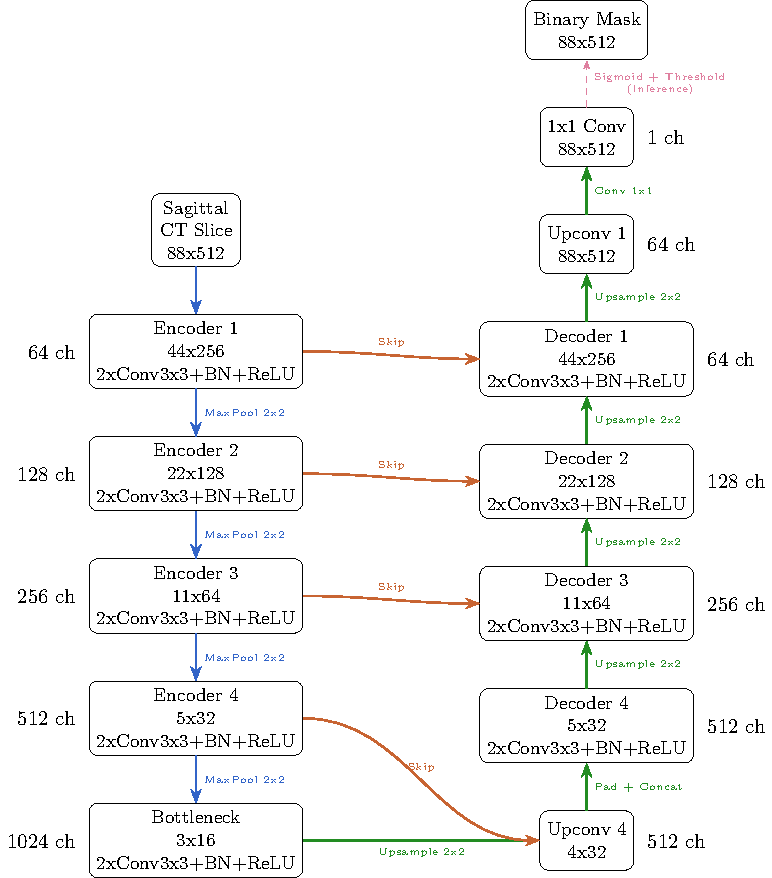
\includegraphics[width=0.8\textwidth,keepaspectratio]{unet.pdf}
    \caption{Architecture of the U-Net model for segmenting kV-CBCT images. The contracting path (left) extracts features, while the expansive path (right) generates precise segmentation masks. Skip connections link the paths to preserve high-resolution details.}
    \label{fig:unet}
\end{figure}

\section{Results}
The segmentation performance was evaluated based on the Dice coefficient, precision, recall, and Hausdorff distance (HD) on the validation data. The filling state is evaluated by measuring the height of the binary segmentation masks in pixels and comparing it with the ground-truth masks.

\begin{table}[H]
    \centering
    \scriptsize
    \begin{tabular}{p{1.8cm}p{2.8cm}p{1.8cm}p{1.8cm}p{3cm}}
      \toprule
      \textbf{Organ} & \textbf{Dice Value\newline (Mean ± SD)} & \textbf{Precision} & \textbf{Recall} & \textbf{Hausdorff Distance\newline (px, Mean ± SD)} \\
      \midrule
      Bladder & 0.9149 ± 0.0852 & 0.8974 & 0.9454 & 9.1419 ± 9.0216 \\
      Rectum & 0.7848 ± 0.1641 & 0.8019 & 0.7958 & 11.5230 ± 10.5643 \\
      \bottomrule
    \end{tabular}
    \caption{Segmentation metrics on validation data (aggregated over 5-fold cross-validation).}
    \label{tab:results}
\end{table}

The high Dice values, precision, and recall, as well as moderate Hausdorff distances, indicate reliable segmentation, with the bladder being segmented more precisely than the rectum, which is attributable to its greater anatomical variability. The loss curves (Fig. \ref{fig:loss_curves}) show that both models achieve stable convergence after approximately 50 epochs.

The segmentation performance is further illustrated by Figures \ref{fig:val_bladder} and \ref{fig:val_rectum}, which show raw sagittal slices, ground-truth masks, and model predictions for 6 patients each (3 with acceptable Dice values and the 3 with the lowest Dice values) in the validation sets for the bladder and rectum models. For the bladder (Fig. \ref{fig:val_bladder}), an error in the ground-truth mask for P132 (third row, middle panel) is visible as the cause of the low Dice value. For P050, the contrast is poor—possibly the patient coughed during acquisition—and the contrast between the bladder and bowel is low, similarly for patient P116. For the rectum (Fig. \ref{fig:val_rectum}), the ground-truth masks appear correct, even in the 3 cases with poor Dice values. For patient P037, the model also detects a portion of the rectum above the ground-truth mask, which reduces the Dice value but is clinically sensible. For patient P052, the rectum is barely depicted in the ground-truth mask and not recognized by the model. For patient P129, the model prediction may be more accurately adapted to anatomical reality than the ground-truth mask, despite a Dice value of 0.62.

\begin{figure}[p]
    \centering
    \begin{subfigure}[b]{0.8\textwidth}
        \centering
        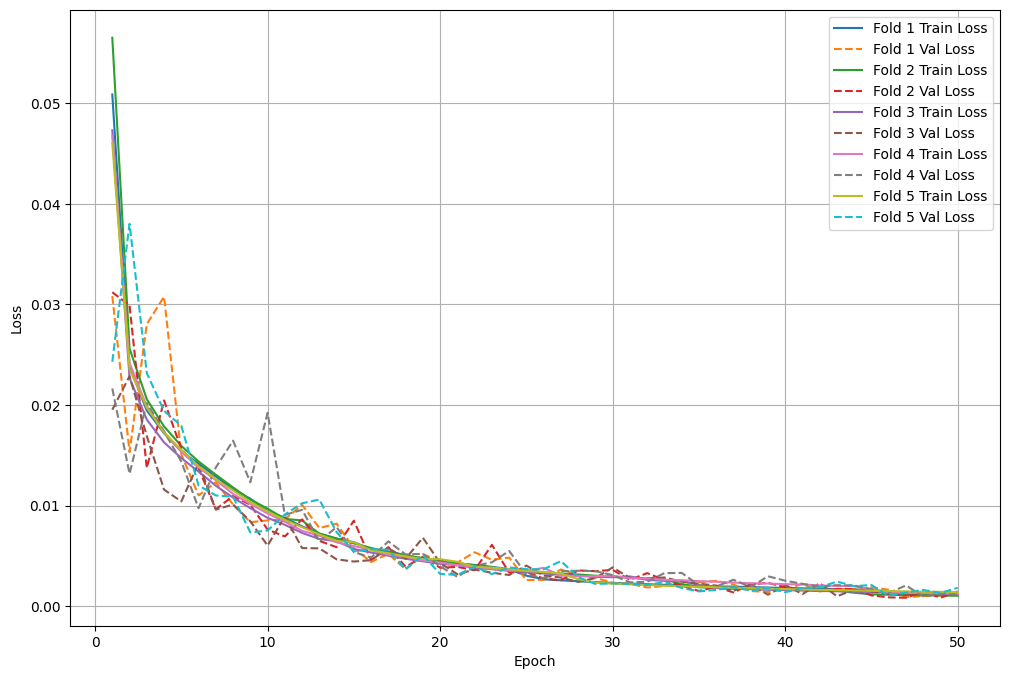
\includegraphics[width=\textwidth,keepaspectratio]{../images/bladder/loss_curves.png}
        \caption{Training and validation losses for the bladder model.}
        \label{fig:loss_curves_bladder}
    \end{subfigure}
    \vspace{0.5cm}
    \begin{subfigure}[b]{0.8\textwidth}
        \centering
        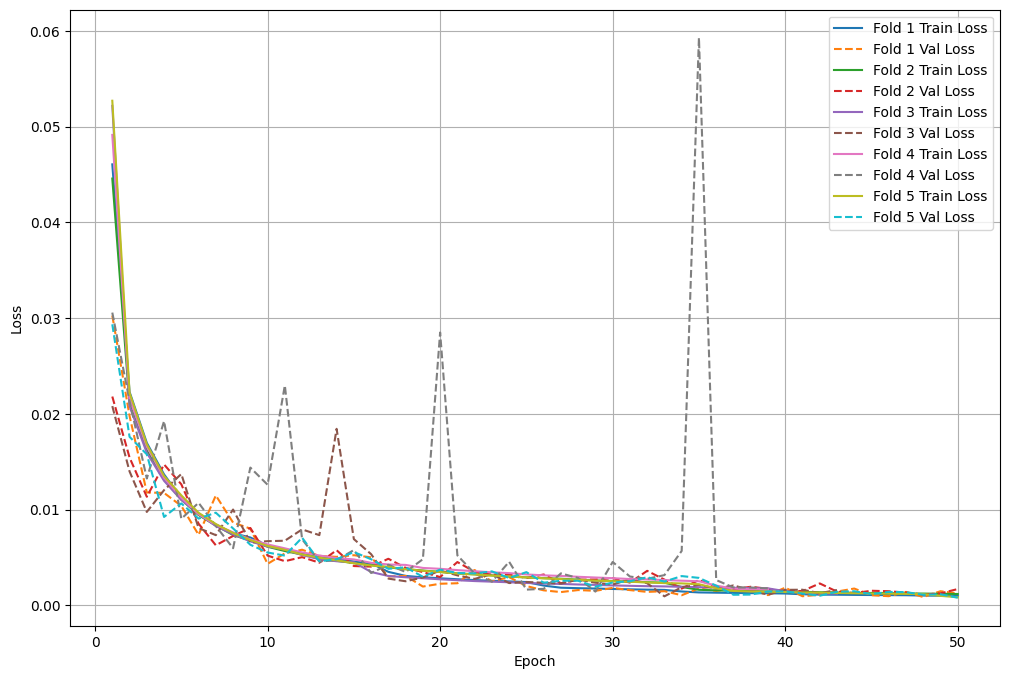
\includegraphics[width=\textwidth,keepaspectratio]{../images/rectum/loss_curves.png}
        \caption{Training and validation losses for the rectum model.}
        \label{fig:loss_curves_rectum}
    \end{subfigure}
    \caption{Progression of training and validation losses over epochs for the bladder and rectum, demonstrating the convergence of the models.}
    \label{fig:loss_curves}
\end{figure}

\begin{figure}[p]
    \centering
    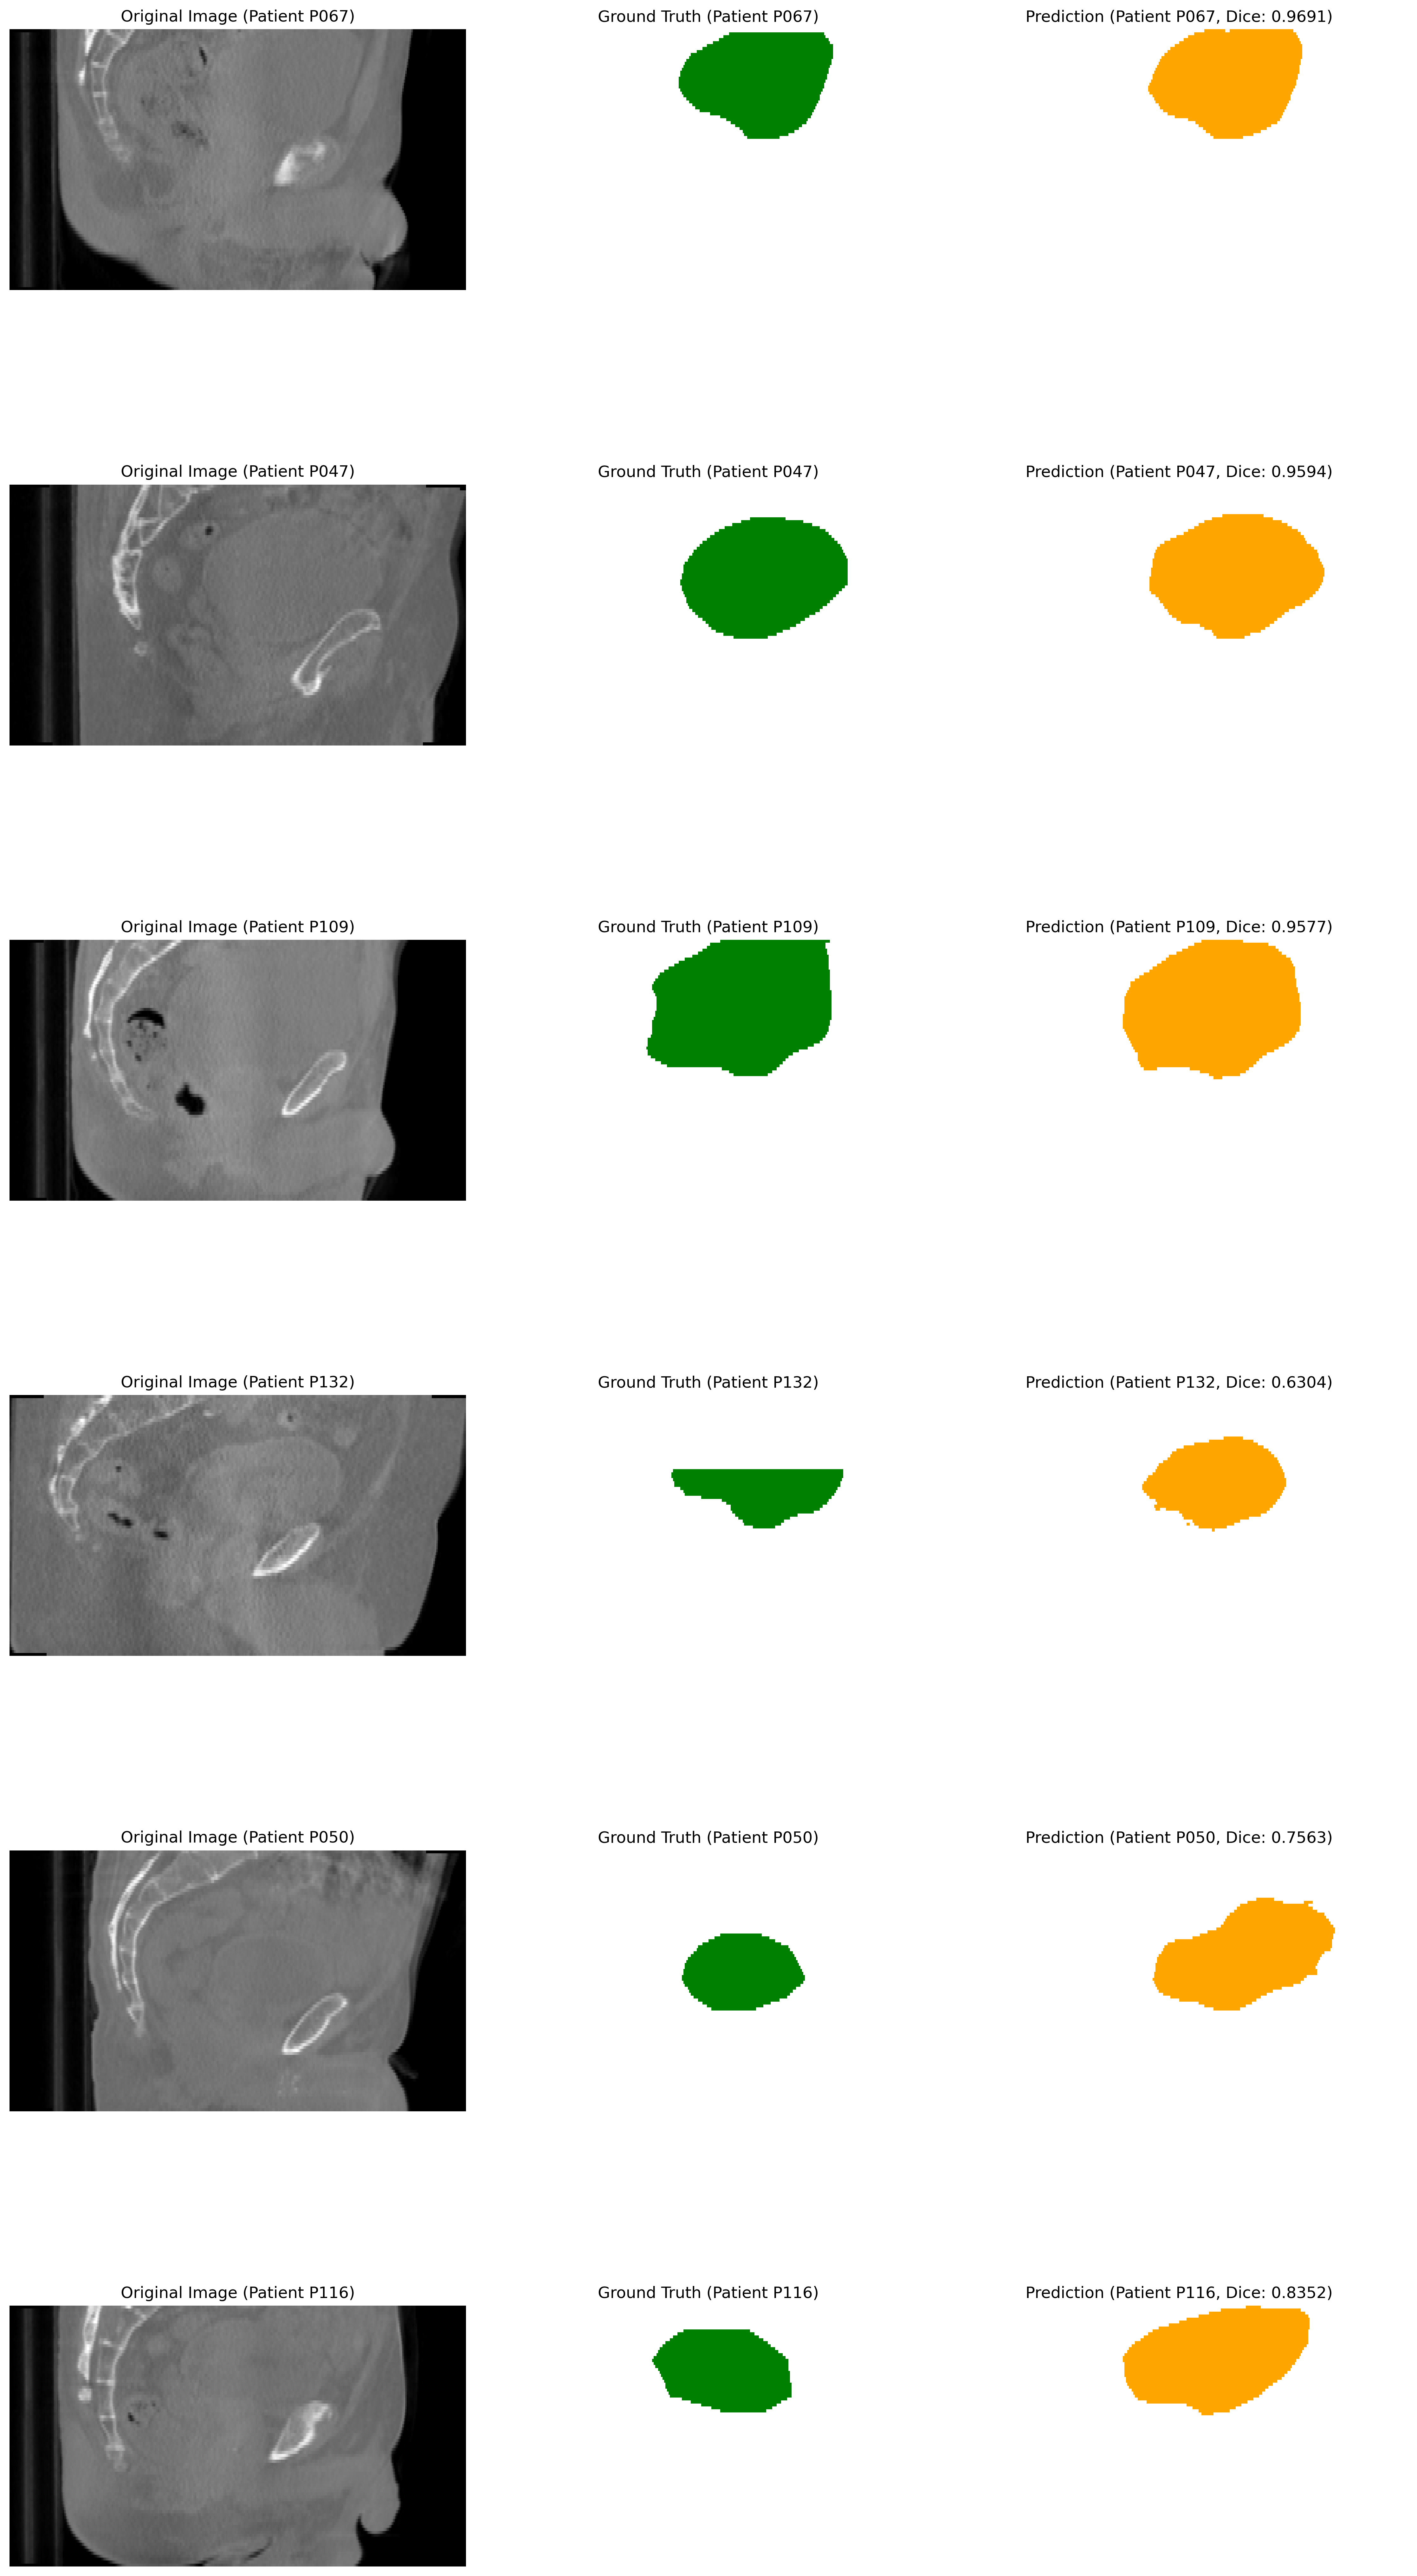
\includegraphics[height=0.9\textheight,keepaspectratio]{../images/bladder/segmentation_grid_6x3.png}
    \caption{Bladder: Panels for validation patients (P067 - Dice 0.97, P047 - Dice 0.96, P109 - 0.96, P132 - Dice 0.63, P050 - Dice 0.76, P116 - Dice 0.84). Left: Original slice; Middle: Ground Truth (green); Right: Prediction (orange).} \label{fig:val_bladder}
\end{figure}

\begin{figure}[p]
    \centering
    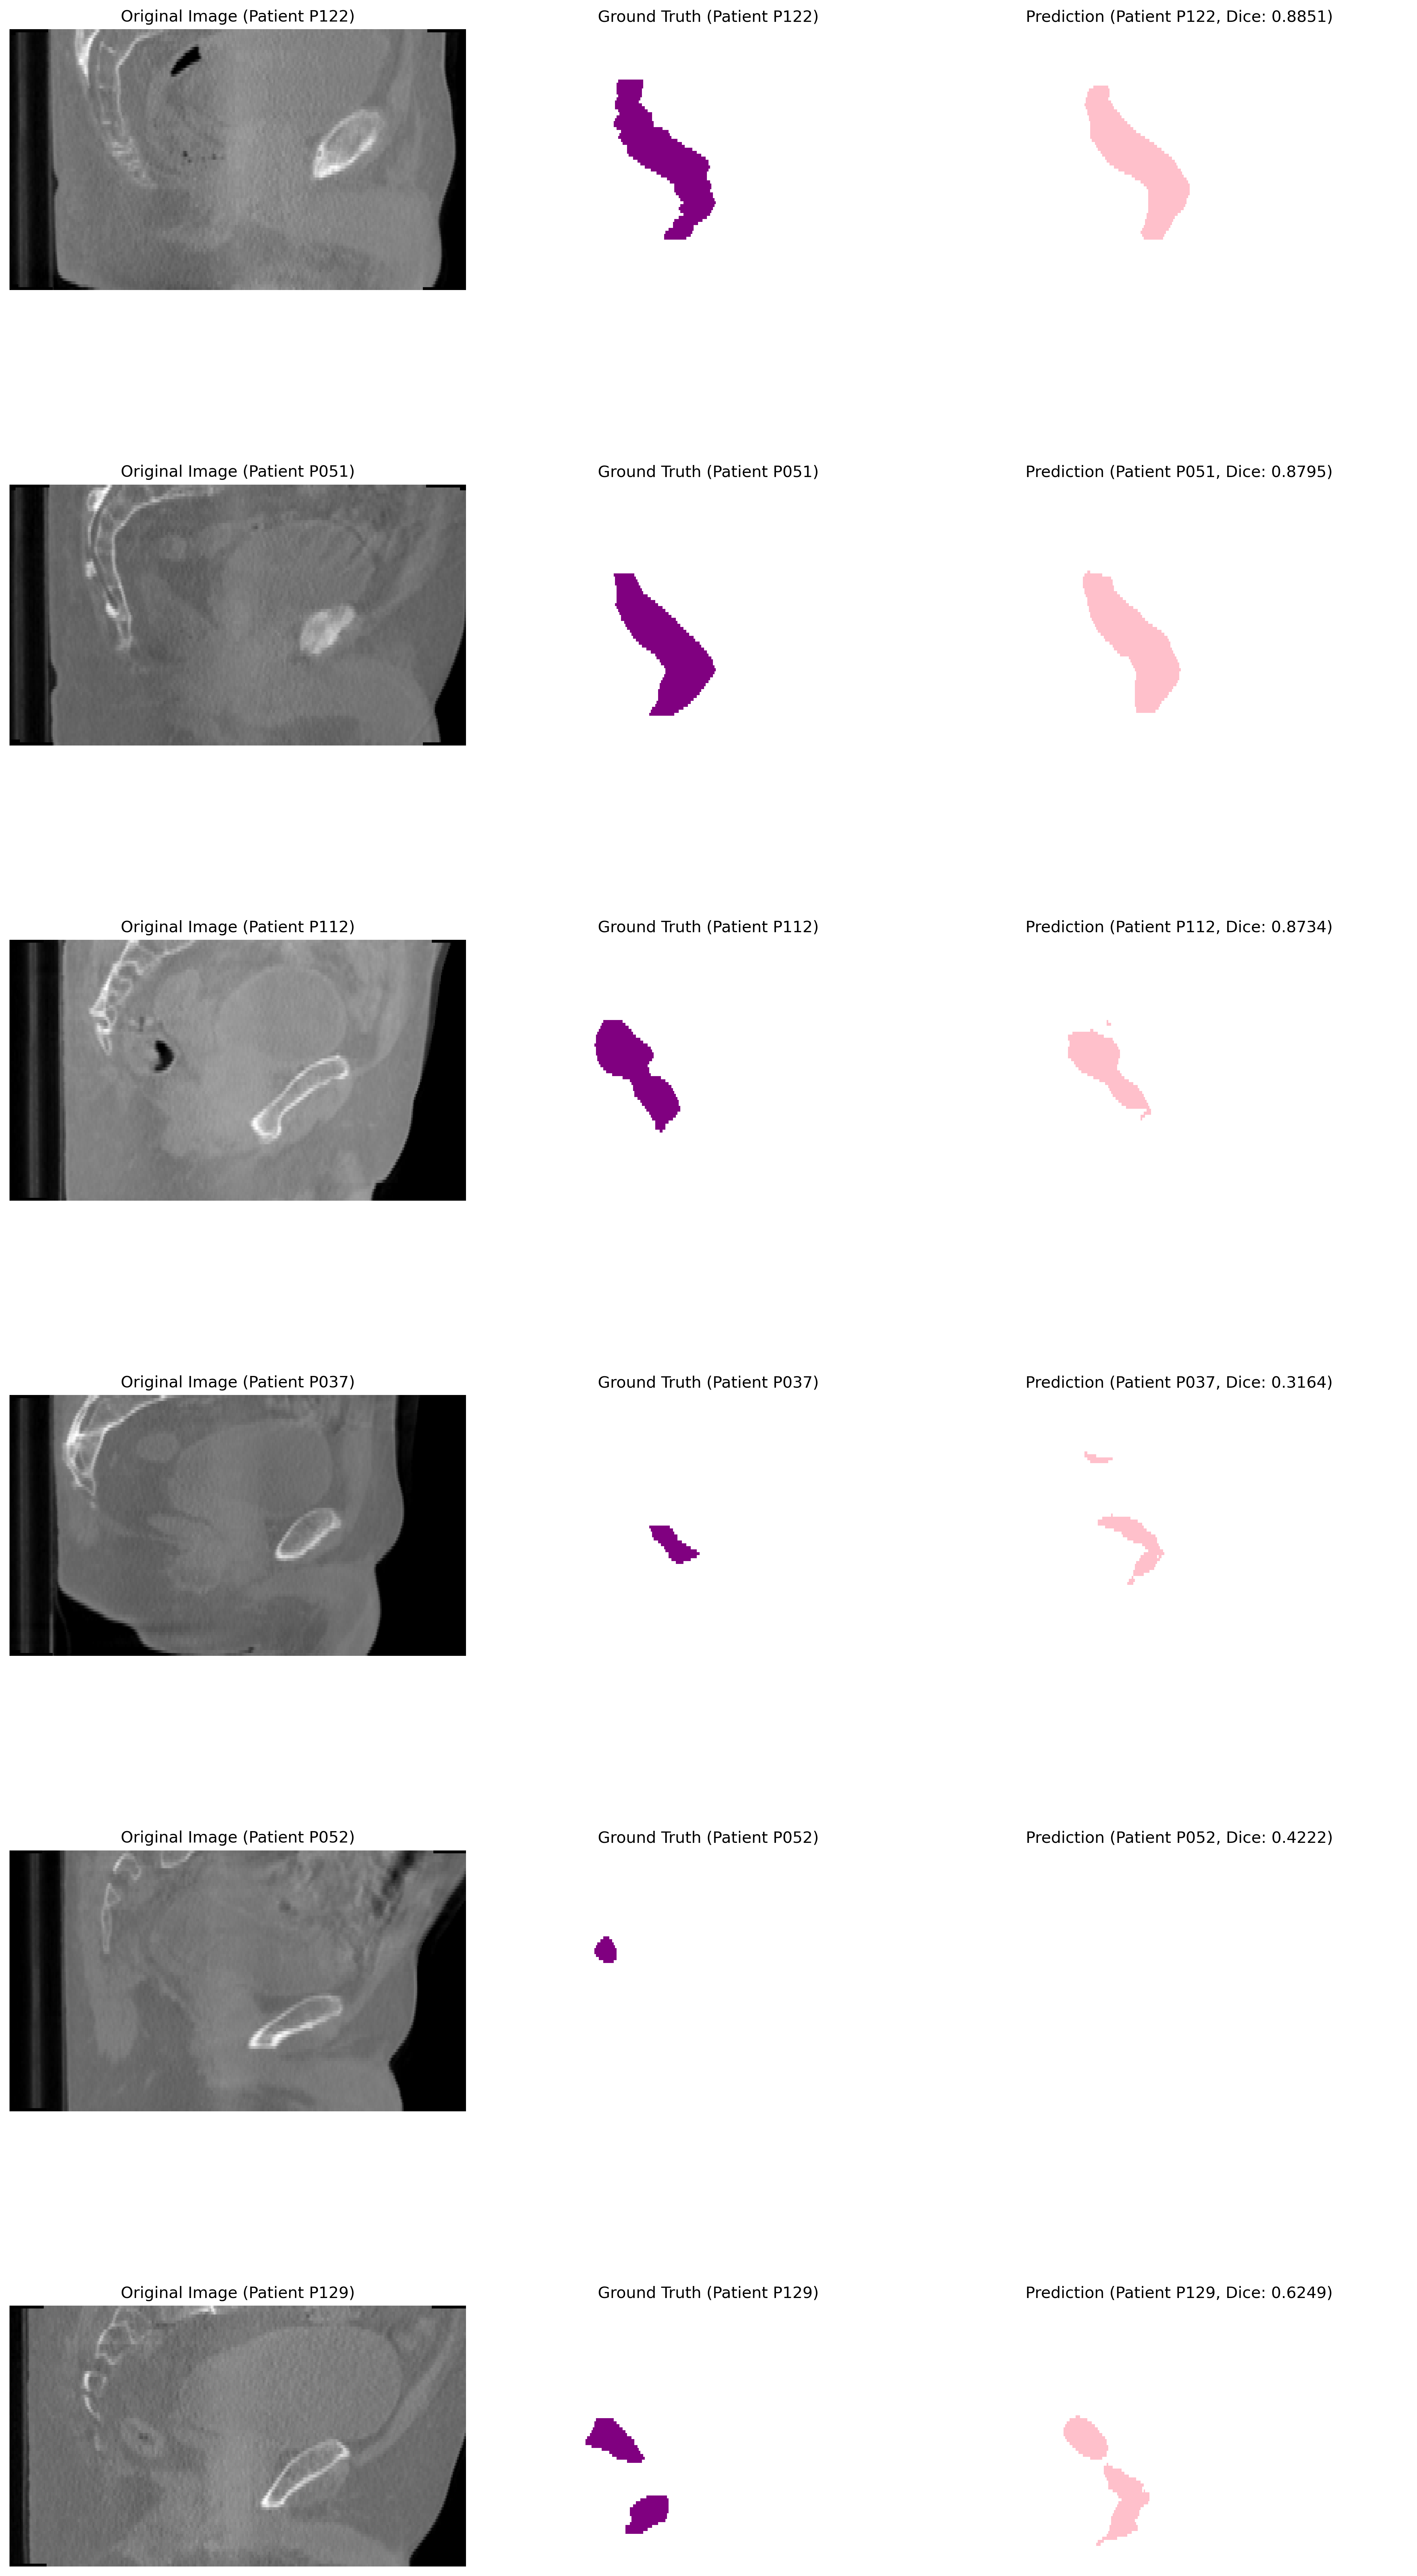
\includegraphics[height=0.9\textheight,keepaspectratio]{../images/rectum/segmentation_grid_6x3.png}
    \caption{Rectum: Panels for validation patients (P122 - Dice 0.89, P051 - Dice 0.88, P112 - Dice 0.87, P037 - Dice 0.31, P052 - Dice 0.42, P129 Dice 0.62). Left: Original slice; Middle: Ground Truth (purple); Right: Prediction (pink).} \label{fig:val_rectum}
\end{figure}

\begin{figure}[p]
    \centering
    \begin{subfigure}[b]{0.8\textwidth}
        \centering
        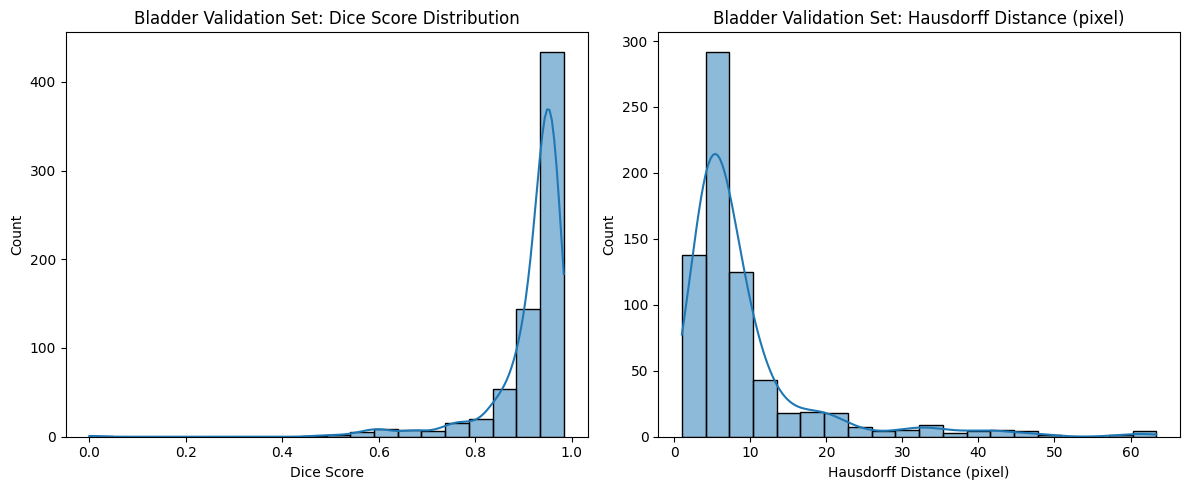
\includegraphics[width=\textwidth,keepaspectratio]{../images/bladder/val_metrics_distribution.png}
        \caption{Metrics distribution for the bladder (Dice and Hausdorff).}
        \label{fig:val_metrics_bladder}
    \end{subfigure}
    \vspace{0.5cm}
    \begin{subfigure}[b]{0.8\textwidth}
        \centering
        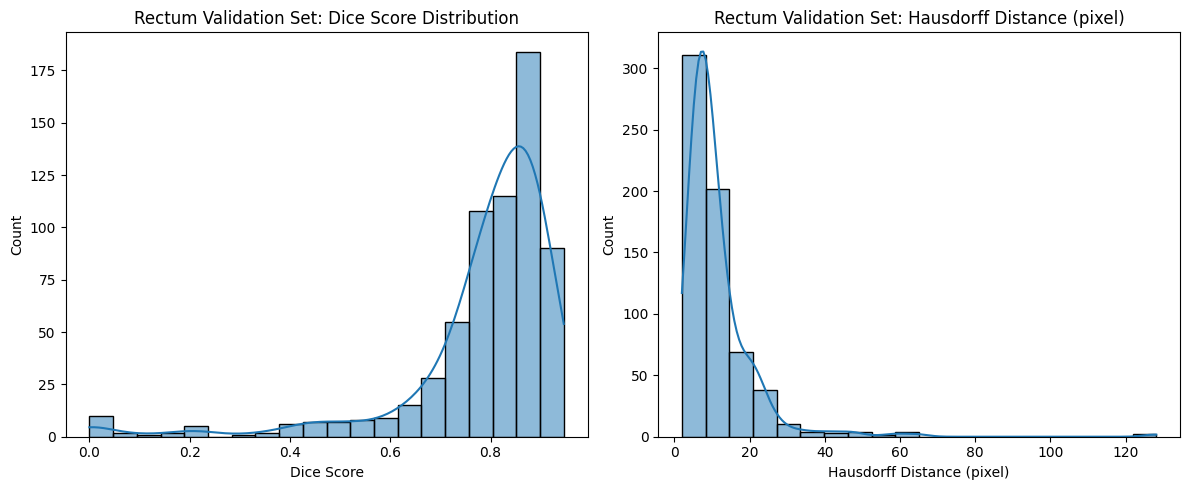
\includegraphics[width=\textwidth,keepaspectratio]{../images/rectum/val_metrics_distribution.png}
        \caption{Metrics distribution for the rectum (Dice and Hausdorff).}
        \label{fig:val_metrics_rectum}
    \end{subfigure}
    \caption{Distribution of validation metrics for bladder and rectum.}
    \label{fig:val_metrics}
\end{figure}

\begin{figure}[p]
    \centering
    \begin{subfigure}[b]{0.8\textwidth}
        \centering
        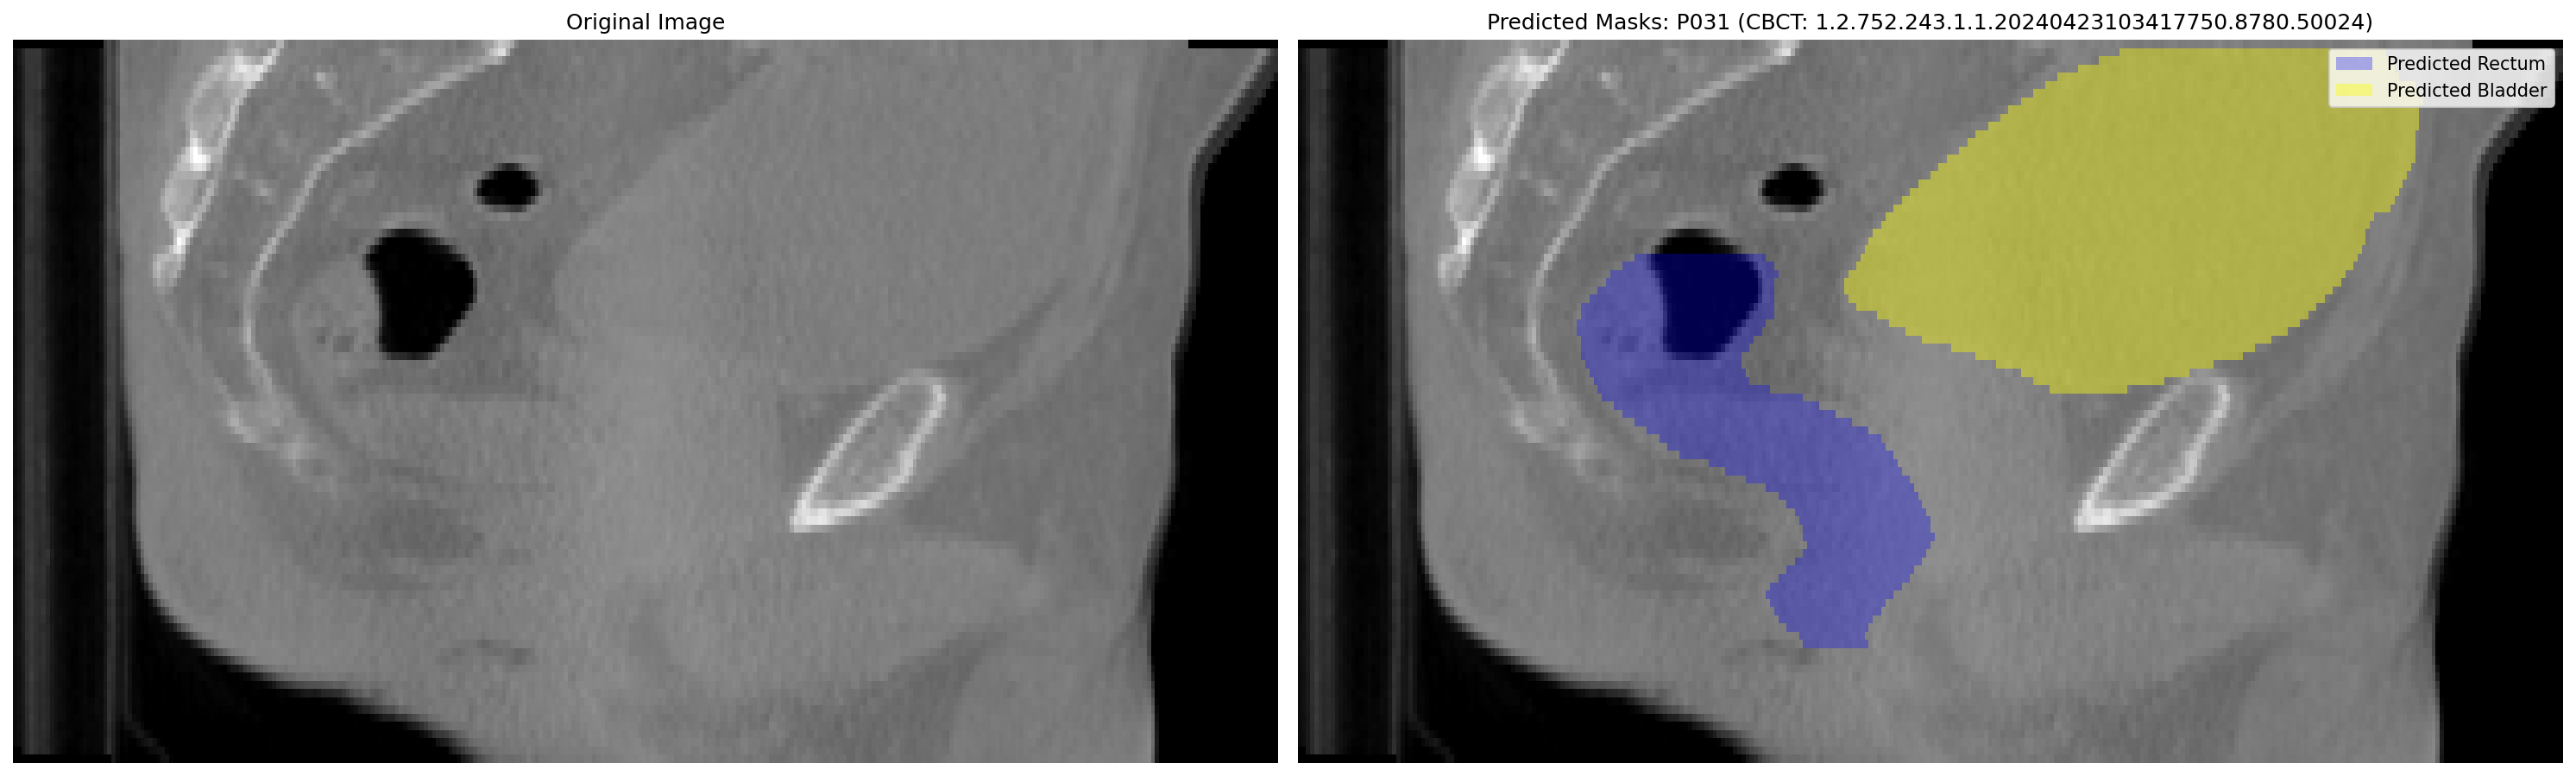
\includegraphics[width=\textwidth,keepaspectratio]{../images/predicted_masks_P031_1.2.752.243.1.1.20240423103417750.8780.50024.png}
        \caption{Overlaid predictions for a common validation patient (Patient 31, CBCT-ID: 1.2.752.243.1.1.20240423103417750.8780.50024).}
        \label{fig:predicted_overlays_p031}
    \end{subfigure}
    \vspace{0.5cm}
    \begin{subfigure}[b]{0.8\textwidth}
        \centering
        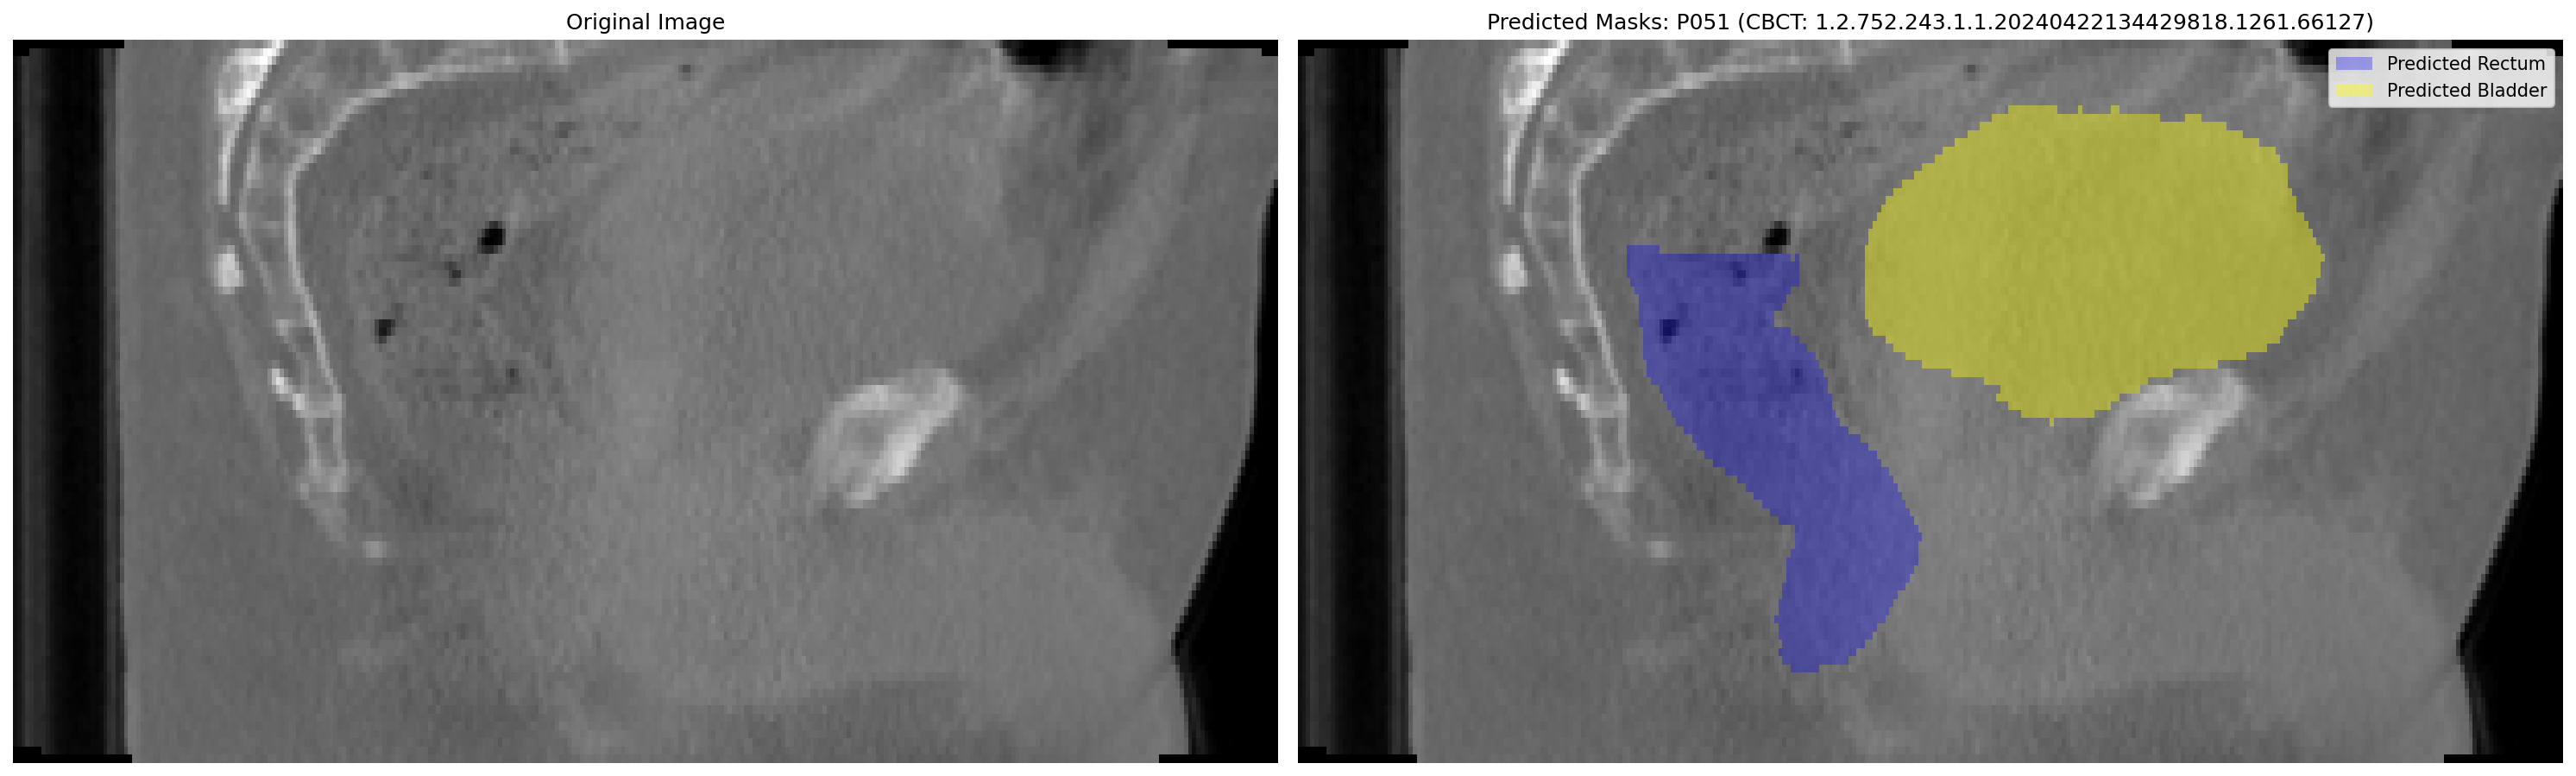
\includegraphics[width=\textwidth,keepaspectratio]{../images/predicted_masks_P051_1.2.752.243.1.1.20240422134429818.1261.66127.png}
        \caption{Overlaid predictions for a common validation patient (Patient 51, CBCT-ID: 1.2.752.243.1.1.20240422134429818.1261.66127).}
        \label{fig:predicted_overlays_p051}
    \end{subfigure}
    \vspace{0.5cm}
    \begin{subfigure}[b]{0.8\textwidth}
        \centering
        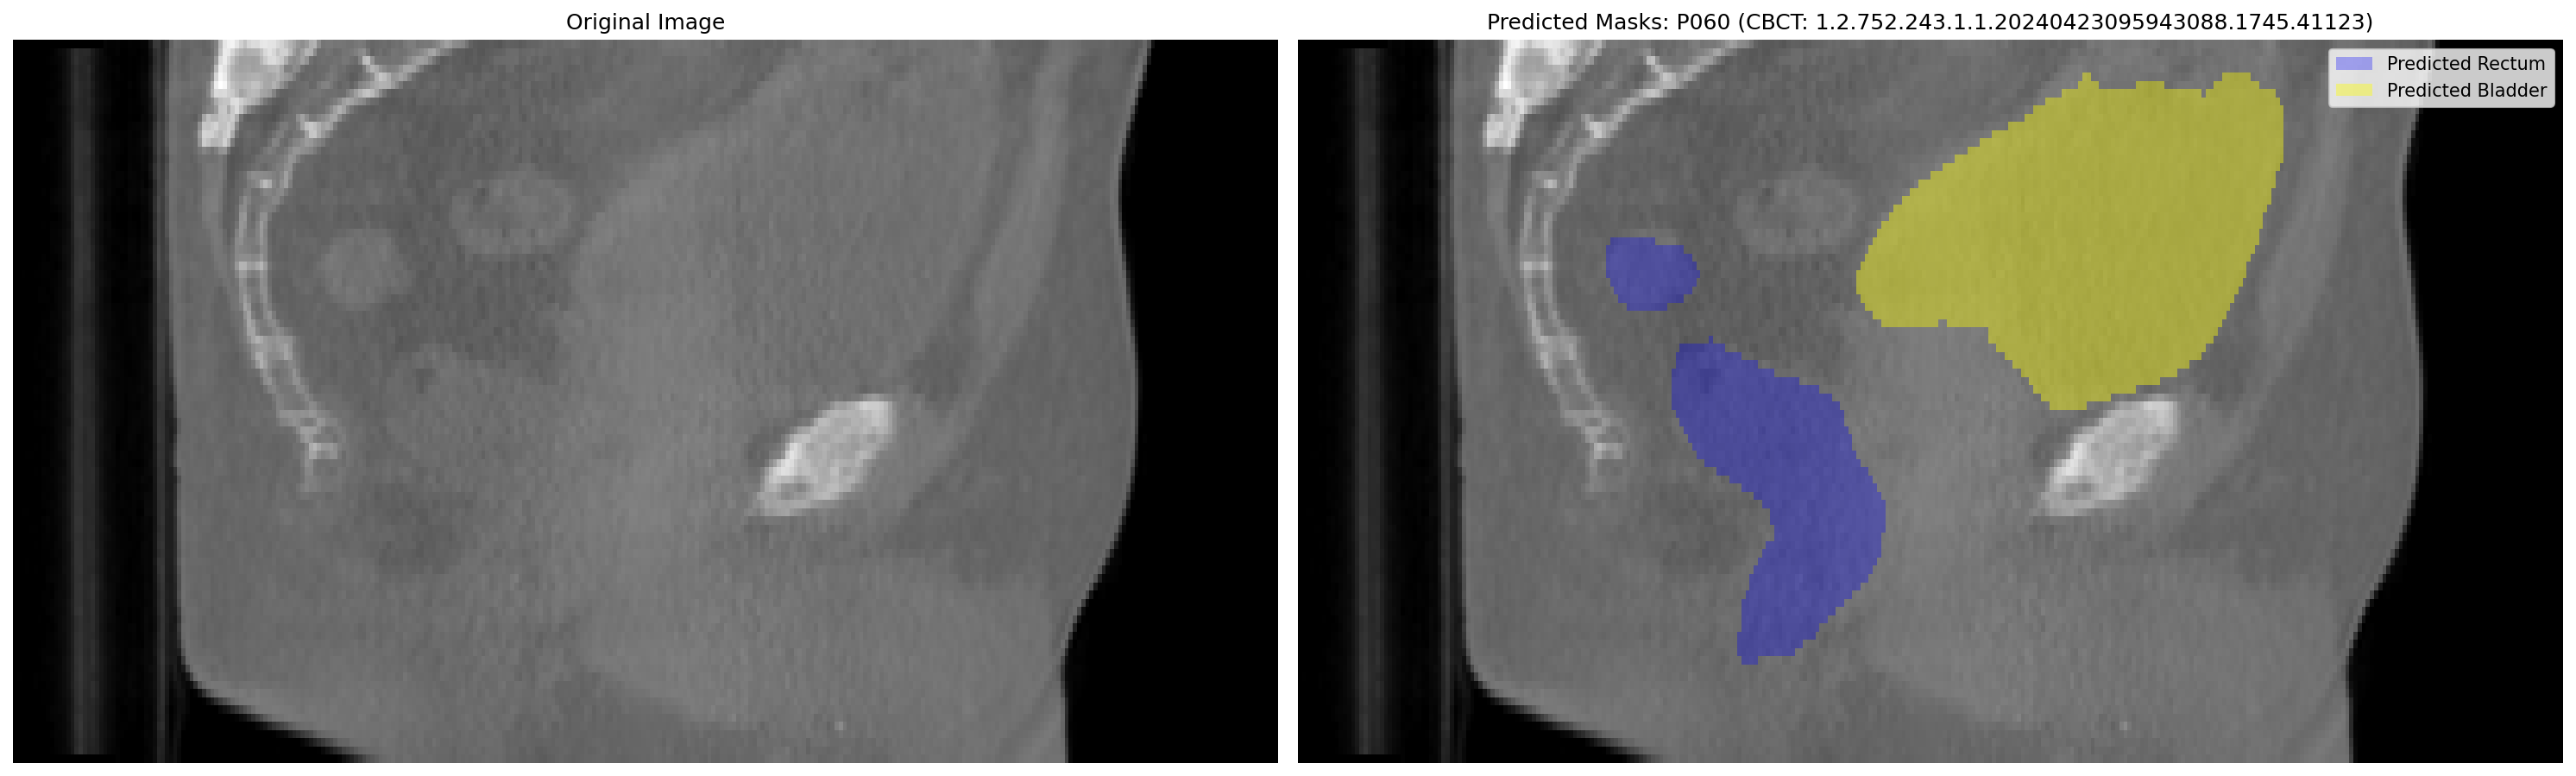
\includegraphics[width=\textwidth,keepaspectratio]{../images/predicted_masks_P060_1.2.752.243.1.1.20240423095943088.1745.41123.png}
        \caption{Overlaid predictions for a common validation patient (Patient 60, CBCT-ID: 1.2.752.243.1.1.20240423095943088.1745.41123).}
        \label{fig:predicted_overlays_p060}
    \end{subfigure}
    \caption{Overlaid model predictions for bladder (yellow) and rectum (blue) exemplarily applied to common validation patients.}
    \label{fig:predicted_overlays}
\end{figure}

\section{Discussion}
The method enables precise segmentation of the bladder and rectum. The Dice value of 0.9149 ± 0.0852 for the bladder and 0.7848 ± 0.1641 for the rectum, combined with Hausdorff distances of 9.1419 ± 9.0216 px and 11.5230 ± 10.5643 px, respectively, provides reliable results for daily use in IGRT. The higher standard deviation for the rectum reflects its greater anatomical variability \citep{rayed2024}. The loss curves (Fig. \ref{fig:loss_curves}) show that both models achieve stable convergence.

The trained models can be executed on a conventional computer in a few seconds (nearly in real time), enabling integration into clinical routine, e.g., as a plugin for the RayStation or Aria system, and making daily verification of organ position or filling practical \citep{antonelli2022}.

In the future, AI-based segmentation could replace the use of fiducials (e.g., gold markers for IGRT) in certain cases, reducing treatment costs and time as well as avoiding risks associated with invasive procedures.

An extension of the model to the entire kV-CBCT volume would enable 3D segmentation of the organs at risk and increase the accuracy and robustness of the method. However, this would require a larger data basis and more computational power. Since the training was performed on a home computer, we prioritized 2D for real-time inference (seconds per image) and clinical feasibility. Future work could test 3D models.

Compared to studies such as \citep{radici2024}, which report Dice values of ~0.90 for the bladder and ~0.85–0.90 for the rectum on CBCT data, our model shows comparable performance for the bladder (0.9149) and slightly lower for the rectum (0.7848), despite the challenge of 2D slices. The lower Dice values for the rectum may be attributable to its complex geometry and filling variations, as also observed in \citep{rayed2024}.

In the future, a multi-organ model could be tested to avoid overlaps and increase consistency \citep{wasserthal2023}. A performance comparison between single- and multi-organ models would be valuable, but inference for both organs individually is seconds-fast, and VRAM requirements are low. Thus, both models can be run simultaneously on consumer hardware—as shown in Fig. \ref{fig:predicted_overlays} (code available on GitHub \citep{rhone_repo}).

Theoretically planned is an alert to the radiation therapist if there is a significant deviation of the model prediction from the ground-truth mask, e.g., a height difference > 10 pixels or an area deviation > 20\%. Whether a height deviation or area deviation is clinically more relevant, and at what threshold an alert is useful, would need to be evaluated in future studies.

The worst results in terms of Dice values occurred with poorly segmented organs, caused by anatomical variations, e.g., truncated images, poor contrast due to image artifacts (e.g., metal implants or movements), or incomplete organ capture in the CT. This indicates limitations in the model's generalizability, particularly with extreme filling states or image artifacts. The analysis of worst-case examples shows that the model tends to over- or under-segment in such cases, which could be addressed by extended augmentation or transfer learning in future iterations.

Limitations of the method include dependence on consistent kV-CBCT parameters as well as information loss due to dimension reduction to 2D. The dataset is homogeneous (no high-risk profiles, data from one device: Elekta Synergy system, kV=120, mAs=650). Anatomical peculiarities such as postoperative states, excessive bowel gas, or implants were rare; model performance in such cases was limited, as the worst-case analysis shows. External validation is essential to test generalizability. Future work could employ transfer learning, extended augmentation, or nnU-Net to improve robustness against variable device properties.

\section{Conclusion}
The AI-based method effectively automates the verification of bladder and rectum filling and offers potential to improve treatment quality and efficiency in IGRT. The high performance metrics and stable convergence of the models (Fig. \ref{fig:loss_curves}) support reliable segmentation of the organs at risk, facilitating their use in clinical practice.

\section{References}
\bibliographystyle{plainnat} 
\bibliography{references} 

\end{document}
